\documentclass{beamer}
\usepackage{amsmath,amssymb,amsthm,verbatim}
\usetheme{Madrid}

\title[Denoising Sound]{Denoising Sound with Discrete Wavelet Transformations}
\subtitle{In Mathematica}
\author{Christopher David Miller}
\institute{Allegheny College}
\date{\today}

\begin{document}
\begin{frame}
    \titlepage
\end{frame}
\begin{frame}
    \frametitle{Digital Sound}
    \begin{figure}
        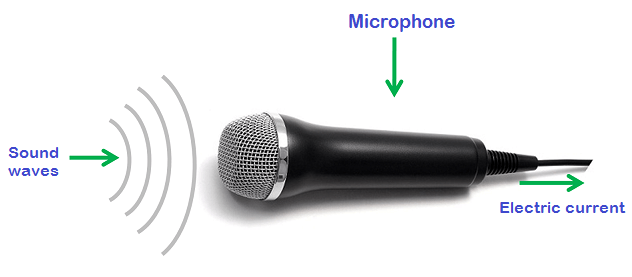
\includegraphics[scale=.5]{soundModel.png}
    \end{figure}
\end{frame}
\begin{frame}
    \frametitle{Digital Sound}
    \begin{columns}
        \begin{columns}
            \column{0.5\textwidth}
           \begin{itemize}
               \item Sampling Rate
               \item Bit Depth
           \end{itemize}
            \column{0.5\textwidth}
            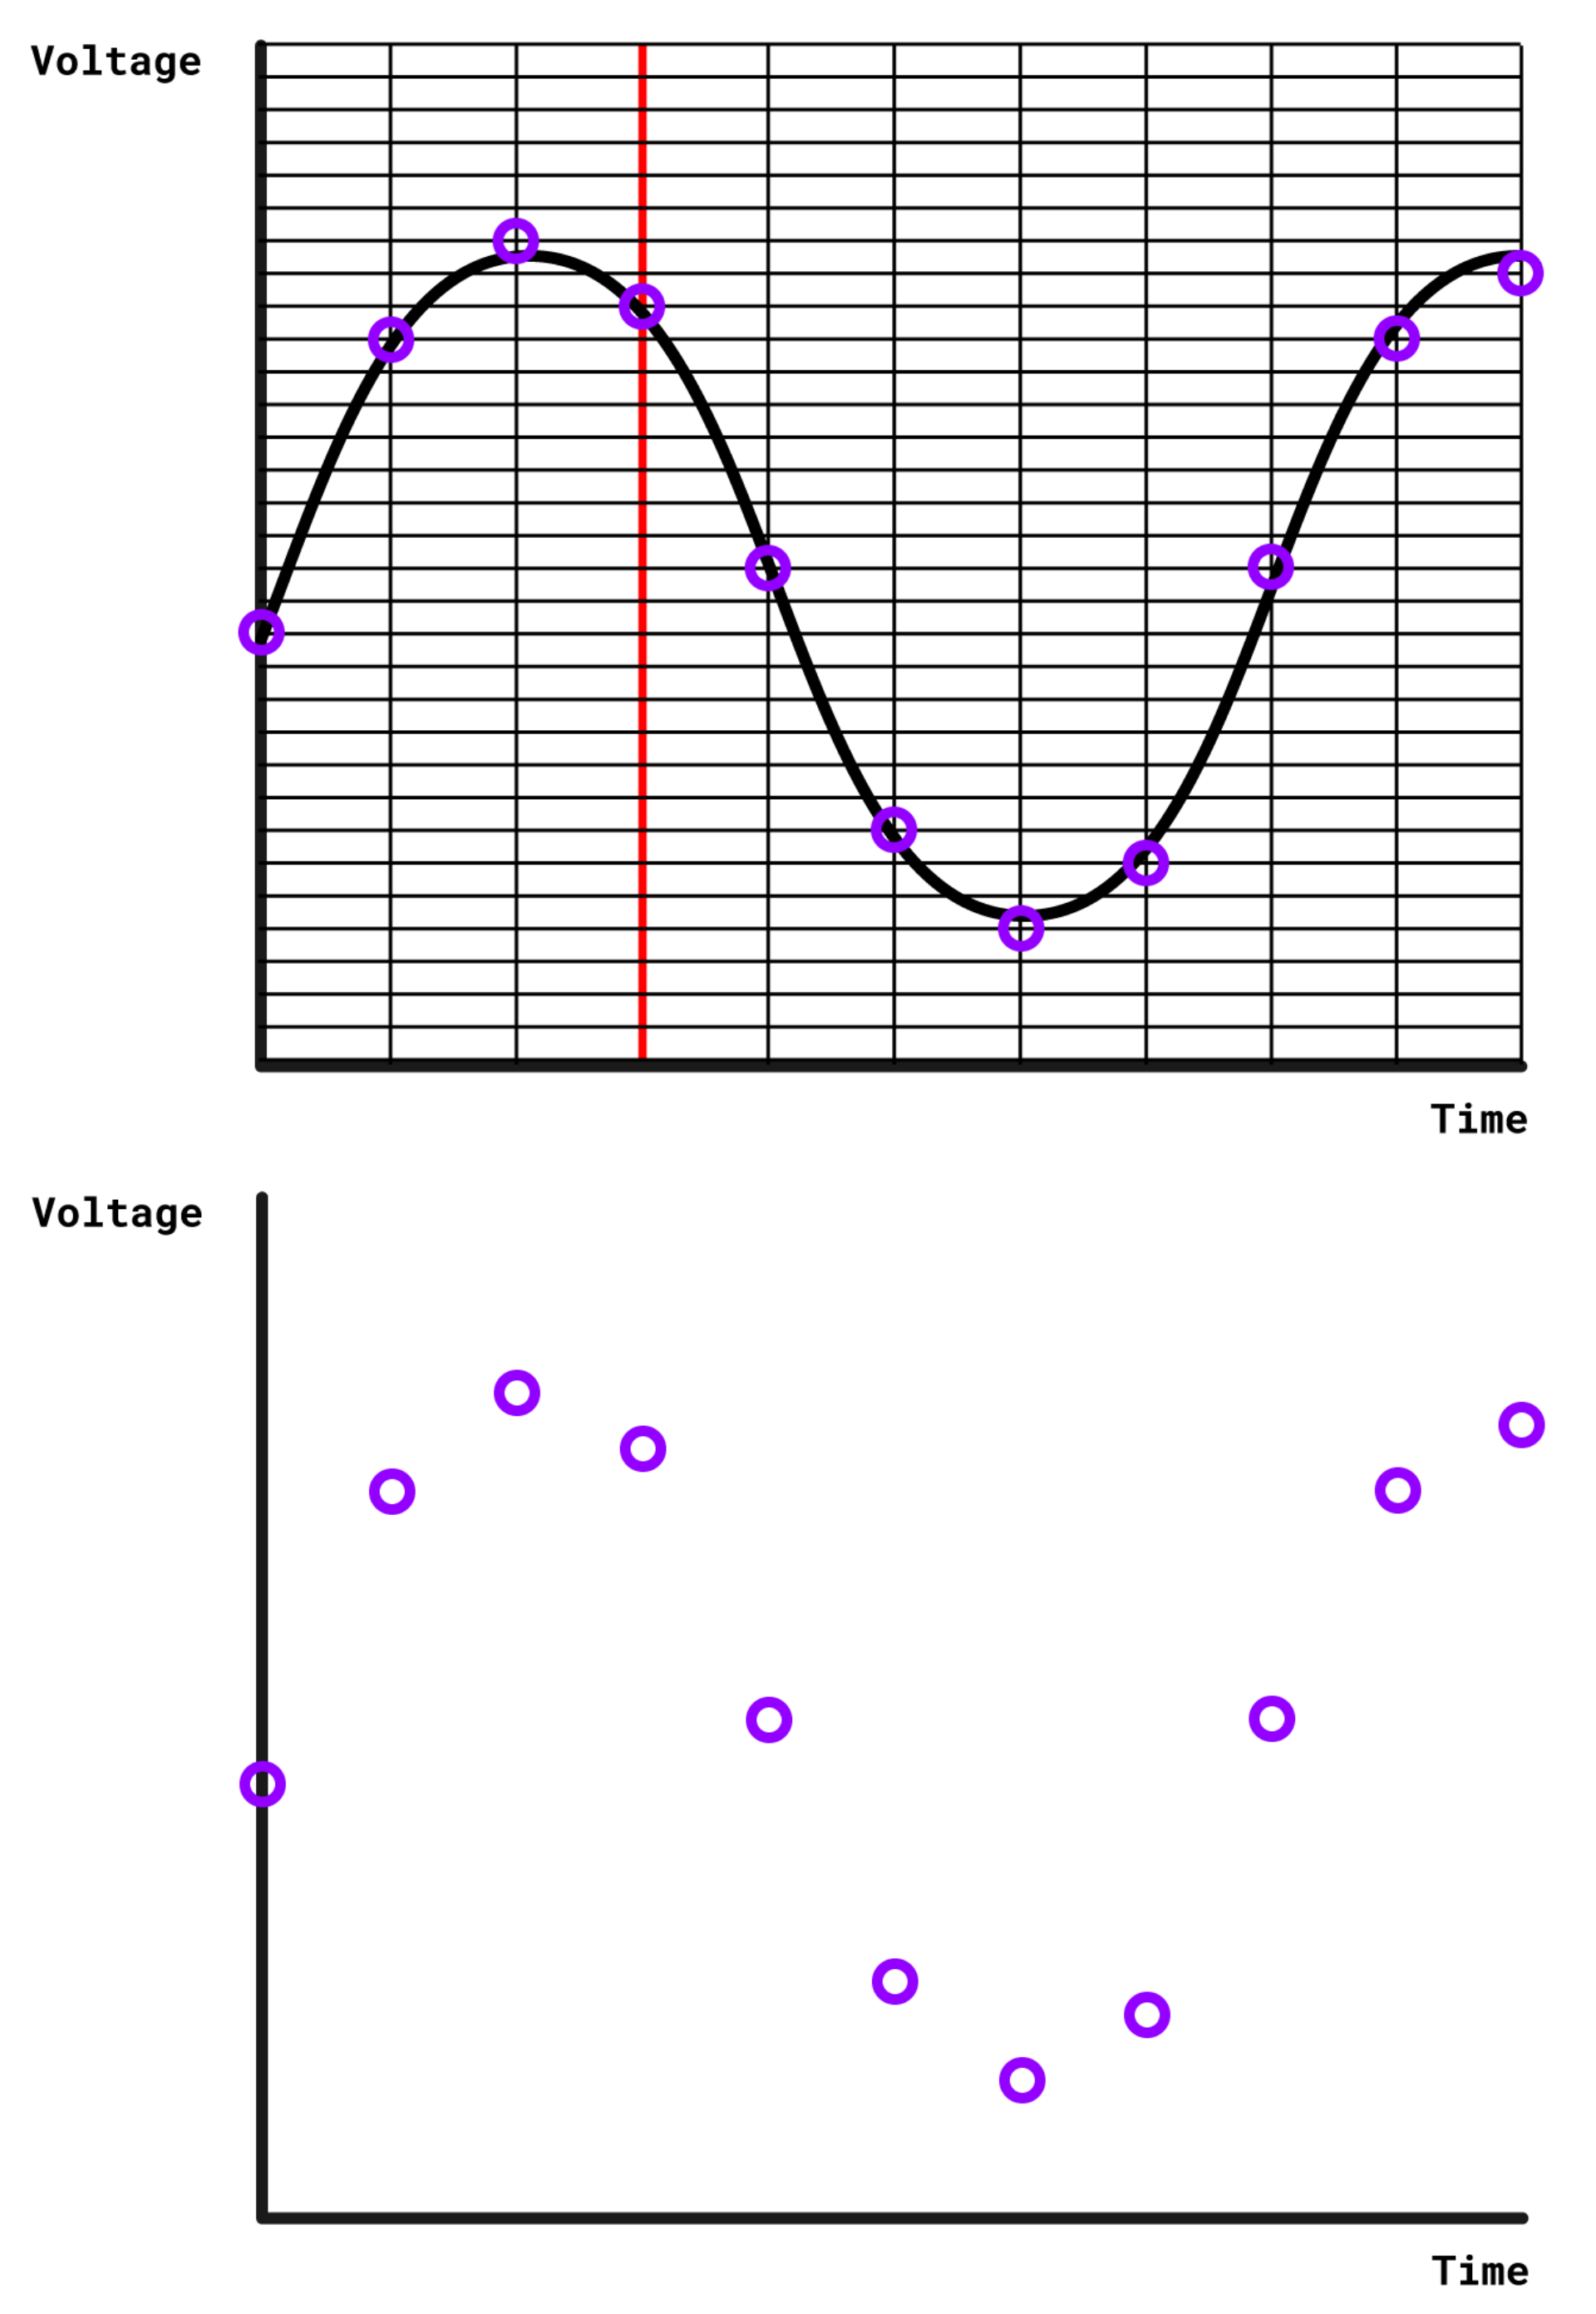
\includegraphics[scale=.1]{voltageGraph.png}
            \end{columns}
    \end{columns}
    
\end{frame}
\begin{frame}
    \frametitle{Sound as an Array}
    To The CODE
\end{frame}
\section{Section 1}
\subsection{sub a}
 

\end{document}